\section{System Core Design}
\subsection{System Design with POR, POW, CLK and BOOT}
\begin{landscape}
  \begin{center}
  \begin{figure}[H]
    
\includegraphics[width=\pdfpagewidth,height=0.65\textheight]{../System-Schematic-Diagrams/Figures/main-unit-and-psu.png}
    \caption{Main Unit with PSU Schematic}
    \label{fig:main-with-psu-schematic-core}
  \end{figure}
  \end{center}
  \begin{center}
  \begin{figure}[H]
    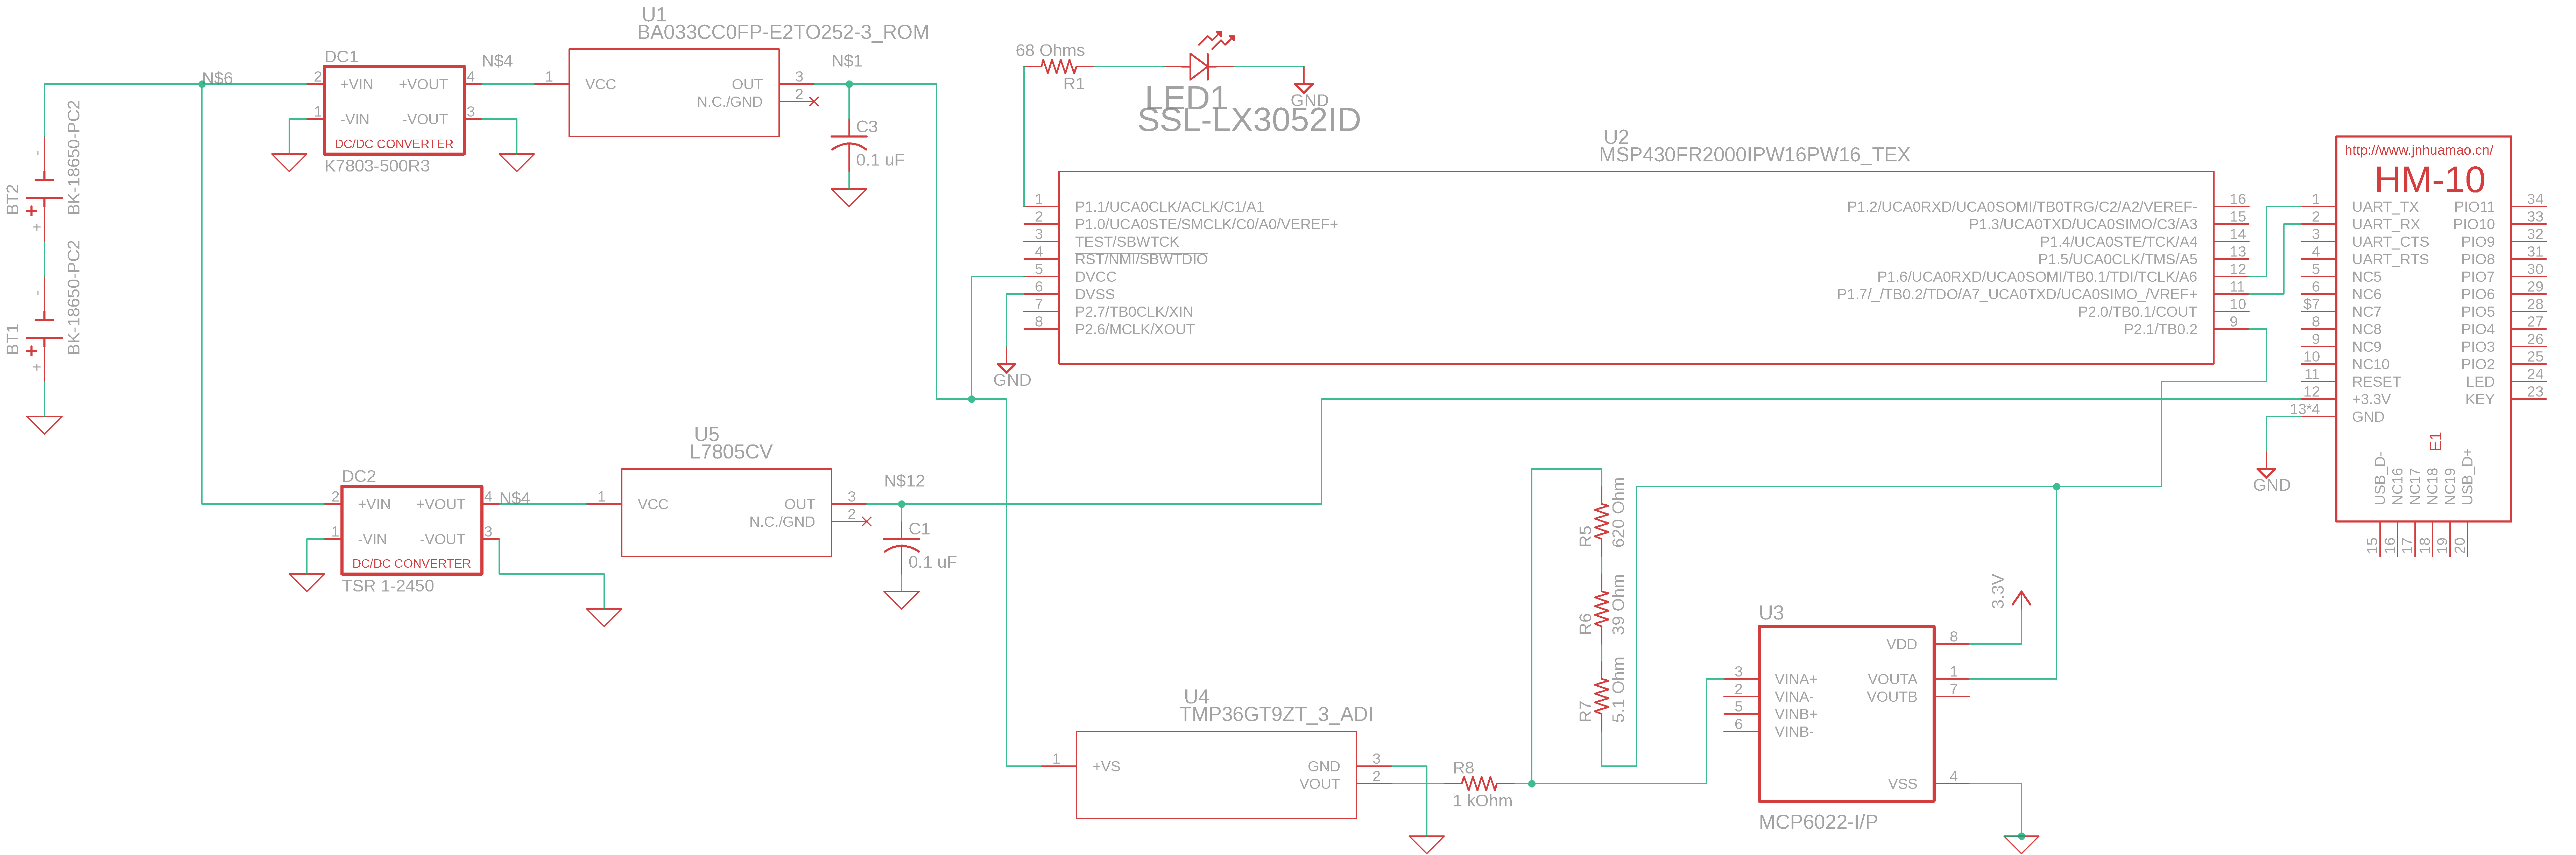
\includegraphics[width=\pdfpagewidth,height=0.65\textheight]{../System-Schematic-Diagrams/Figures/sub-unit-and-psu.png}
    \caption{Sub Unit with PSU Schematic}
    \label{fig:sub-with-psu-schematic-core}
  \end{figure}
  \end{center}
\end{landscape}
Note: For this design used the MSP430FR2311 development board, POR, POW, CLK and BOOT are included within the development board for both the main and sub unit.
\subsection{System Core Demonstration}
\subsection{Integration Plan}
\subsubsection{Integration Order and Verification Plan}
\begin{enumerate}
  \item Connect both MSP430FR2311 to the 3.3\si{\V} supply with their respective power supplies.
  \item Connect the LEDs with their respective resistors with the MCU pins and ground.
        \begin{itemize}
         \item To verify that the MSP430FR2311s are working, an LED will be lit by a push button in order by the MCU.
        \end{itemize}
  \item Connect the power sense pin to a GPIO of the main unit.
        \begin{itemize}
         \item  To verify that this is working, an LED shall be lit by the MCU when power is absent and off when power is present.
        \end{itemize}
  \item Connect the HM-10 Bluetooth modules to the 5\si{\V} supply of their respective power supplies.
  \item Connect the UART pins from the MCU to the HM-10s.
        \begin{itemize}
         \item To verify this, we shall check if it can send a ``Hello World'' to a serial monitor.
        \end{itemize}
  \item Connect the external temperature sensor to the 3.3\si{\V} supply and connect the output pin to a ADC pin on the MCU.
        \begin{itemize}
         \item In order to verify that this is working, we shall use the debugger to see the ADC registers.
        \end{itemize}
\end{enumerate}
\subsubsection{Member Logistic}
\begin{enumerate}
  \item Enrique will complete the UART integration with the Bluetooth module for the HM-10 for both TXD and RXD interrupts.
  \item Guillermo will complete the ADC integration with thee temperature sensor plus op amp.
  \item Enrique will give the main unit prototype to Fabio.
  \item Guillermo will give the sub unit prototype to Fabio.
  \item Fabio will verify that the sub unit can communicate with the main unit.
  \item Fabio will verify that the host computer can communicate with a host computer.
  \item Fabio will integrate the main and sub units with their respective power supplies.
\end{enumerate}
